% Assorted constructs from real talks: long titles, buttons, logos, lettered lists.
\documentclass{beamer}
\usetheme{Boadilla}
\usepackage{enumerate}
\graphicspath{{img/}}
\title{Miscellaneous}
\author{Test Author}
\logo{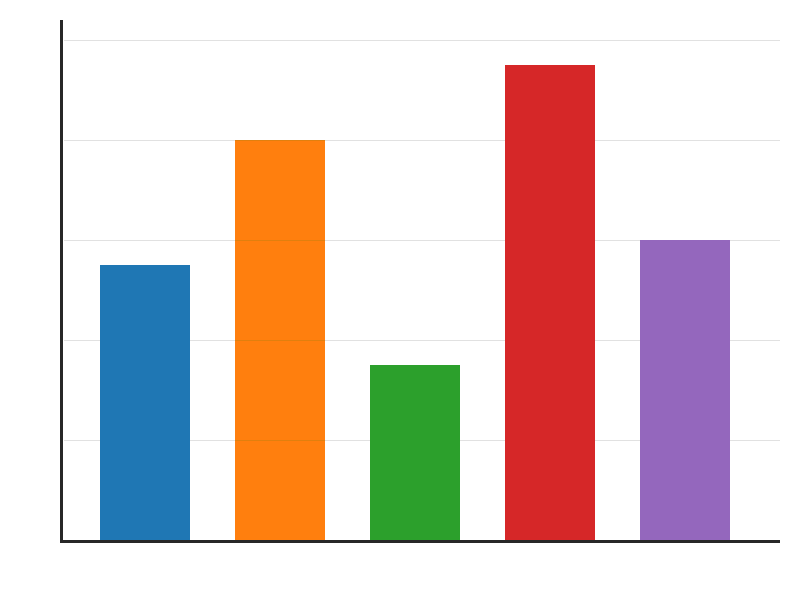
\includegraphics[height=0.6cm]{plot.png}}

\begin{document}

\begin{frame}{A rather long frame title that does not fit on a single line of the slide}
  \begin{enumerate}[a)]
    \item First lettered item
    \item Second lettered item
  \end{enumerate}
  \begin{itemize}
    \item Outer item
    \begin{enumerate}
      \item Inner numbered one
      \item Inner numbered two
    \end{enumerate}
  \end{itemize}
\end{frame}

\begin{frame}{Buttons and small print}
  \hyperlink{last}{\beamergotobutton{Jump to the end}}

  \vspace{1em}
  {\tiny This tiny print is a disclaimer that nobody reads, but it is still text.}

  \begin{verse}
    Roses are red,\\
    violets are blue.
  \end{verse}
\end{frame}

\begin{frame}[label=last]{The end}
  \centering\Large Done.
\end{frame}

\end{document}
